%************************************************
\chapter{Results}\label{ch:results}
%************************************************
This chapter presents results from the end application.

\section{Translations}
We begin by demonstrating how a few sentences are parsed into an abstract syntax which is linearized into all possible concrete syntaxes. The input is shown in the first box in each figure (with input language as a comment) and the result in second (larger) box. The result of a translation is JSON-data, given by the application.

The first five figures shows the most simplest translations. They include all subjects and all types of names. Each one contains a subject, one verb and one name of a certain type.
\newline
\newline

\autoref{fig:result1} shows that the word \texttt{Java} is of the type \texttt{Skill}.

\begin{figure}[H]
\begin{terminal}
-- EnglishRGL
people who know Java
\end{terminal}
\begin{json-small}
[
 {
  'ast': 'InstrucInternal People (Know_R (MkSkill (MkSymb "Java")))',
  'linearizations': [
   {
    'query': 'people who know Java',
    'language': 'InstrucsEngConcat'
   },
   {
    'query': 'people who know Java',
    'language': 'InstrucsEngRGL'
   },
   {
    'query': 'select?q=*:*&wt=json&fq= object_type : Person AND KNOWS : ( Java )',
    'language': 'InstrucsSolr'
   },
   {
    'query': 'personer som kan Java',
    'language': 'InstrucsSweRGL'
   }
  ]
 }
]
\end{json-small}
\caption{Translation including \texttt{people} and a name of type \texttt{Skill}\label{fig:result1}}
\end{figure}

\autoref{fig:result2} shows that the word \texttt{London} is of the type \texttt{Location}.

\begin{figure}[H]
\begin{terminal}
-- English RGL
people who work in London
\end{terminal}
\begin{json-small}
[
 {
  'ast': 'InstrucInternal People (WorkIn_R (MkLocation (MkSymb "London")))',
  'linearizations': [
   {
    'query': 'people who work in London',
    'language': 'InstrucsEngConcat'
   },
   {
    'query': 'people who work in London',
    'language': 'InstrucsEngRGL'
   },
   {
    'query': 'select?q=*:*&wt=json&fq= object_type : Person AND WORKS_IN : ( London )',
    'language': 'InstrucsSolr'
   },
   {
    'query': 'personer som arbetar i London',
    'language': 'InstrucsSweRGL'
   }
  ]
 }
]
\end{json-small}
\caption{Translation including \texttt{people} and a name of type \texttt{Location}\label{fig:result2}}
\end{figure}

\autoref{fig:result3} shows that the word \texttt{Amnesty} is of the type \texttt{Organization}.

\begin{figure}[H]
\begin{terminal}
-- EnglishRGL
people who work with Amnesty
\end{terminal}
\begin{json-small}
[
 {
  'ast': 'InstrucInternal People (WorkWith_R (MkOrganization (MkSymb "Amnesty")))',
  'linearizations': [
   {
    'query': 'people who work with Amnesty',
    'language': 'InstrucsEngConcat'
   },
   {
    'query': 'people who work with Amnesty',
    'language': 'InstrucsEngRGL'
   },
   {
    'query': 'select?q=*:*&wt=json&fq= object_type : Person AND WORKS_WITH : ( Amnesty )',
    'language': 'InstrucsSolr'
   },
   {
    'query': 'personer som arbetar med Amnesty',
    'language': 'InstrucsSwe'
   }
  ]
 }
]
\end{json-small}
\caption{Translation including \texttt{people} and a name of type \texttt{Organization}\label{fig:result3}}
\end{figure}

\autoref{fig:result4} shows that the word \texttt{Solr} is of the type \texttt{Module}.

\begin{figure}[H]
\begin{terminal}
-- EnglishRGL
customers who use Solr
\end{terminal}
\begin{json-small}
[
 {
  'ast': 'InstrucExternal Customer (UseExt_R (MkModule (MkSymb "Solr")))',
  'linearizations': [
   {
    'query': 'customers who use Solr',
    'language': 'InstrucsEngConcat'
   },
   {
    'query': 'customers who use Solr',
    'language': 'InstrucsEngRGL'
   },
   {
    'query': 'select?q=*:*&wt=json&fq= object_type : Organization AND USES : ( Solr )',
    'language': 'InstrucsSolr'
   },
   {
    'query': 'kunder som använder Solr',
    'language': 'InstrucsSwe'
   }
  ]
 }
]
\end{json-small}
\caption{Translation including \texttt{customer} and a name of type \texttt{Module}\label{fig:result4}}
\end{figure}

Similarly, also \autoref{fig:result5} shows that the word \texttt{Solr} is of the type \texttt{Module}.

\begin{figure}[H]
\begin{terminal}
-- EnglishRGL
projects who use Solr
\end{terminal}
\begin{json-small}
[
 {
  'ast': 'InstrucResource Project (UseRes_R (MkModule (MkSymb "Solr")))',
  'linearizations': [
   {
    'query': 'projects who use Solr',
    'language': 'InstrucsEngConcat'
   },
   {
    'query': 'projects who use Solr',
    'language': 'InstrucsEngRGL'
   },
   {
    'query': 'select?q=*:*&wt=json&fq= object_type : Project AND USES : ( Solr )',
    'language': 'InstrucsSolr'
   },
   {
    'query': 'projekt som använder Solr',
    'language': 'InstrucsSwe'
   }
  ]
 }
]
\end{json-small}
\caption{Translation including \texttt{project} and a name of type \texttt{Module}\label{fig:asts-depths}}
\end{figure}

\autoref{fig:translation-java-python} shows how the applications handles the boolean operator \emph{and}. The application handles the case for \emph{or} similarly.

\begin{figure}[H]
\begin{terminal}
-- EnglishRGL
people who know Java and Python
\end{terminal}
\begin{json-small}
[
 {
  'ast': 'InstrucInternal People (Know_R (And_S (MkSkill (MkSymb "Java")) 
                                                      (MkSkill (MkSymb "Python"))))',
  'linearizations': [
   {
    'query': 'people who know Java and Python',
    'language': 'InstrucsEngConcat'
   },
   {
    'query': 'people who know Java and Python',
    'language': 'InstrucsEngRGL'
   },
   {
    'query': 'select?q=*:*&wt=json&fq= object_type : Person AND 
                                                KNOWS : ( ( Java ) AND ( Python ) )',
    'language': 'InstrucsSolr'
   },
   {
    'query': 'personer som kan Java och Python',
    'language': 'InstrucsSwe'
   }
  ]
 }
]
\end{json-small}
\caption{Translation including \texttt{people} and two names of the type \texttt{Skill}\label{fig:translation-java-python}}
\end{figure}

\autoref{fig:translation-ambig} shows how the application handles an ambiguous instruction. Two abstract syntax trees are seen in the result, as there are two ways of interpreting the instruction. The different interpretations can be modelled as follows: \emph{people who know (Java and Python) or Haskell} or \emph{people who know Java and (Python or Haskell)}.

\begin{figure}[H]
\begin{terminal}
-- EnglishRGL
people who know Java and Python or Haskell
\end{terminal}
\begin{json-small}
[
 {
  'ast': 'InstrucInternal People (Know_R (Or_S (And_S (MkSkill (MkSymb "Java")) 
                       (MkSkill (MkSymb "Python"))) (MkSkill (MkSymb "Haskell"))))',
  'linearizations': [
   {
    'query': 'people who know Java and Python or Haskell',
    'language': 'InstrucsEngConcat'
   },
   {
    'query': 'people who know Java and Python or Haskell',
    'language': 'InstrucsEngRGL'
   },
   {
    'query': 'select?q=*:*&wt=json&fq= object_type : Person AND 
                      KNOWS : ( ( ( Java ) AND ( Python ) ) OR ( Haskell ) )',
    'language': 'InstrucsSolr'
   },
   {
    'query': 'personer som kan Java och Python eller Haskell',
    'language': 'InstrucsSwe'
   }
  ]
 },
 {
  'ast': 'InstrucInternal People (Know_R (And_S (MkSkill (MkSymb "Java")) 
                      (Or_S (MkSkill (MkSymb "Python")) (MkSkill (MkSymb "Haskell")))))',
  'linearizations': [
   {
    'query': 'people who know Java and Python or Haskell',
    'language': 'InstrucsEngConcat'
   },
   {
    'query': 'people who know Java and Python or Haskell',
    'language': 'InstrucsEngRGL'
   },
   {
    'query': 'select?q=*:*&wt=json&fq= object_type : Person AND 
                      KNOWS : ( ( Java ) AND ( ( Python ) OR ( Haskell ) ) )',
    'language': 'InstrucsSolr'
   },
   {
    'query': 'personer som kan Java och Python eller Haskell',
    'language': 'InstrucsSwe'
   }
  ]
 }
]
\end{json-small}
\caption{Translation of an ambiguous instruction involving \texttt{people} and three names of the type \texttt{Skill}\label{fig:translation-ambig}}
\end{figure}

\section{Suggestions}
This section shows how the application reacts to input before the user has chosen to translate the instruction. Each figure shows an image of how the application suggest valid sentences from a partial instruction.

\autoref{fig:suggestions-people} shows suggestions based on the first word in a valid sentence.

\begin{figure}[H]
\includegraphics[scale=0.6,keepaspectratio,valign=t]{./gfx/people.png}
\caption{Suggestions based on the word \texttt{people} by using EnglishRGL or EnglishConcat\label{fig:suggestions-people}}
\end{figure}

\autoref{fig:suggestions-who-know} shows that it is possible to use a combination of words to retrieve suggestions. It also demonstrates that the words do not have to be the first words in an instruction.

\begin{figure}[H]
\includegraphics[scale=0.6,keepaspectratio,valign=t]{./gfx/who_know.png}
\caption{Suggestions based on the words \texttt{who know} by using EnglishRGL or EnglishConcat\label{fig:suggestions-who-know}}
\end{figure}

The next four figures shows how it is possible to retreive suggestions based on only names.

\begin{figure}[H]
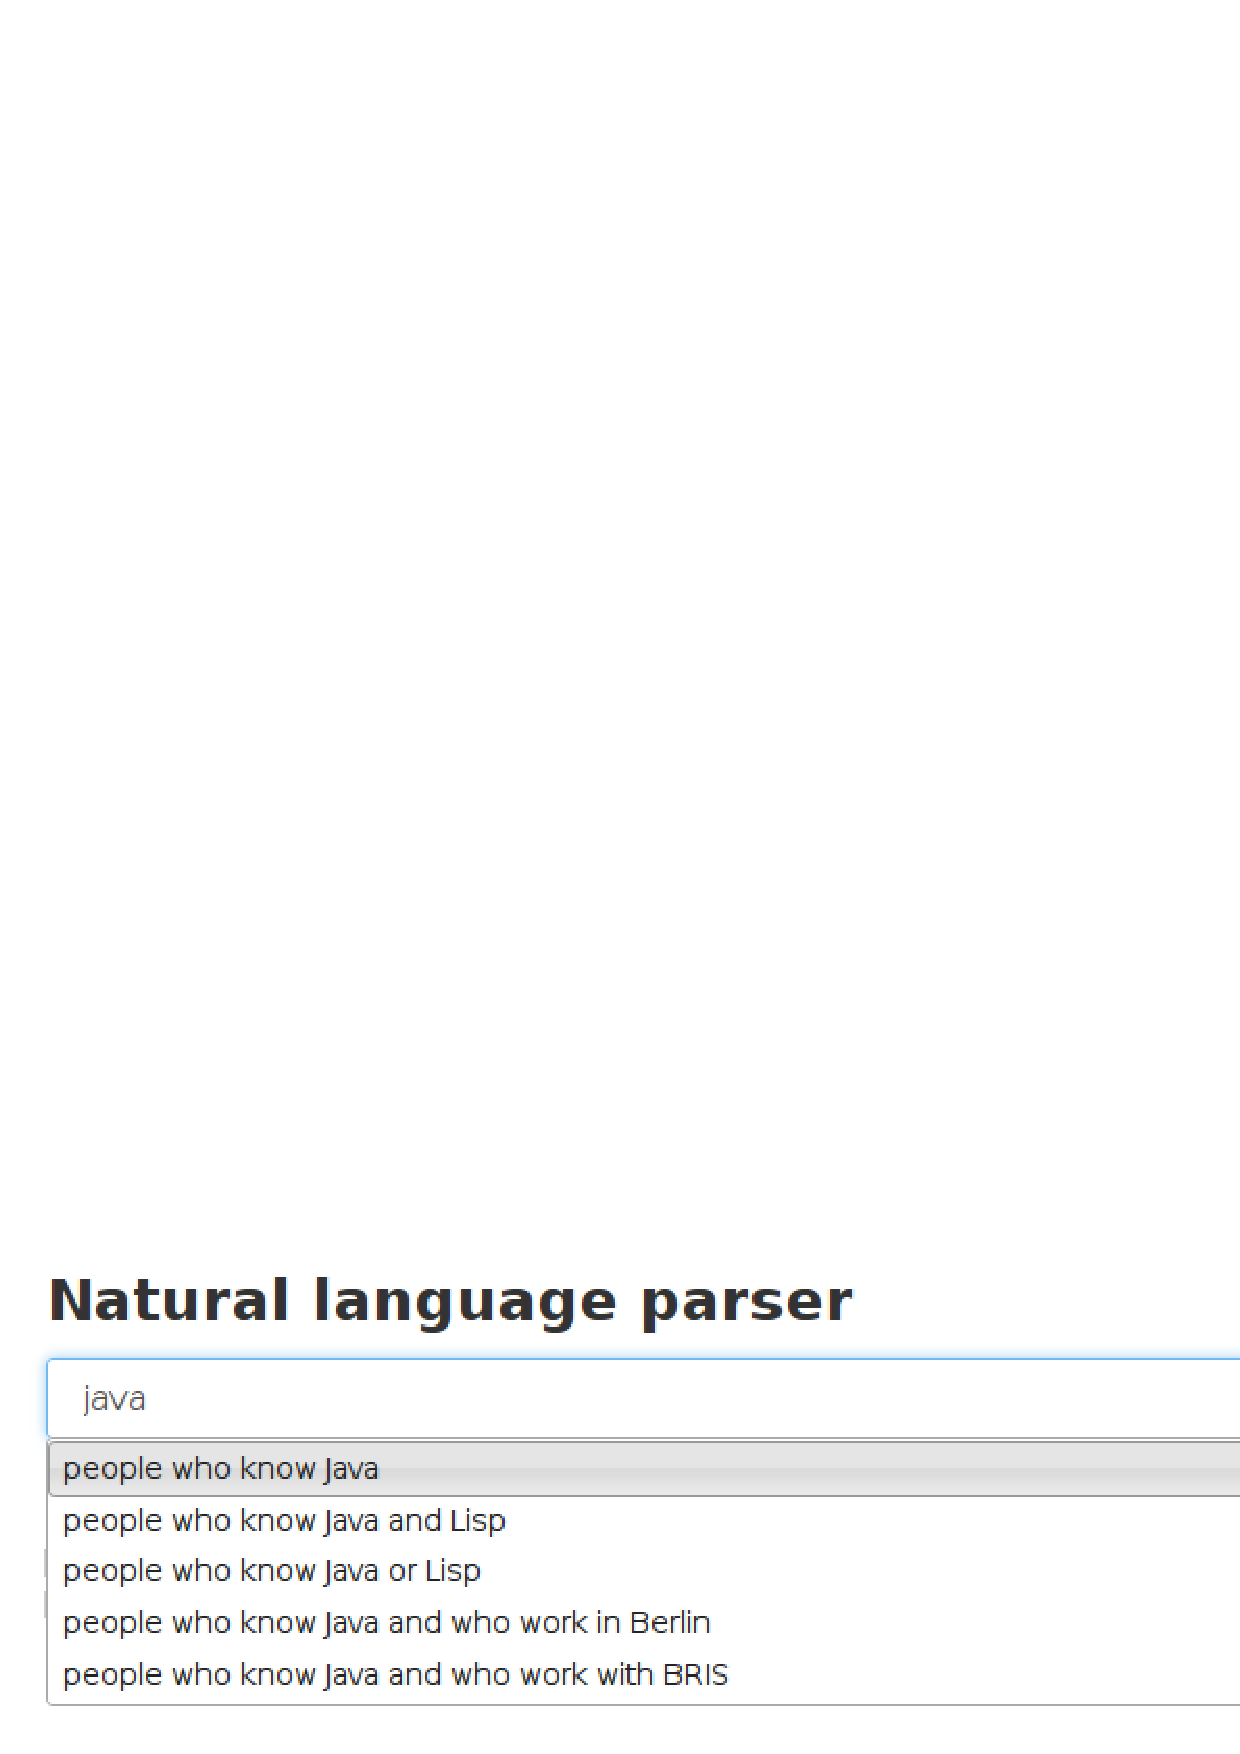
\includegraphics[scale=0.6,keepaspectratio,valign=t]{./gfx/java.png}
\caption{Suggestions based on a name of type Skill by using EnglishRGL or EnglishConcat\label{fig:name-skill}}
\end{figure}

\begin{figure}[H]
\includegraphics[scale=0.6,keepaspectratio,valign=t]{./gfx/london.png}
\caption{Suggestions based on a name of type Location by using EnglishRGL or EnglishConcat\label{fig:name-location}}
\end{figure}

\begin{figure}[H]
\includegraphics[scale=0.6,keepaspectratio,valign=t]{./gfx/amnesty.png}
\caption{Suggestions based on a name of type Organization by using EnglishRGL or EnglishConcat\label{fig:name-organization}}
\end{figure}

\begin{figure}[H]
\includegraphics[scale=0.6,keepaspectratio,valign=t]{./gfx/solr.png}
\caption{Suggestions based on a name of type Module by using EnglishRGL or EnglishConcat\label{fig:name-module}}
\end{figure}

\autoref{fig:java-python} shows suggestions based on two names of the same type.

\begin{figure}[H]
\includegraphics[scale=0.6,keepaspectratio,valign=t]{./gfx/java_python.png}
\caption{Suggestions based on two names  of type Skill by using EnglishRGL or EnglishConcat\label{fig:java-python}}
\end{figure}

\autoref{fig:haskell-london} shows that names do not have to be of the same type to suggest relevant instructions.

\begin{figure}[H]
\includegraphics[scale=0.6,keepaspectratio,valign=t]{./gfx/haskell-london.png}
\caption{Suggestions based on two names of different types by using EnglishRGL or EnglishConcat\label{fig:haskell-london}}
\end{figure}

\autoref{fig:persons} shows how we can use the word \texttt{persons} in order to get suggestions. The word \texttt{persons} does not exist in any suggestion, but as it is a synonym to \texttt{people}, the application suggest relevant instructions.

\begin{figure}[H]
\includegraphics[scale=0.6,keepaspectratio,valign=t]{./gfx/persons.png}
\caption{Synonyms based on a synonym by using EnglishRGL or EnglishConcat\label{fig:persons}}
\end{figure}

Also \autoref{fig:that} shows how we can get suggestions based on a synonym. However, only EnglishConcat gives suggestions based on the word \emph{that}.

\begin{figure}[H]
\includegraphics[scale=0.6,keepaspectratio,valign=t]{./gfx/that.png}
\caption{Synonyms based on a synonym by using EnglishConcat\label{fig:that}}
\end{figure}

\autoref{fig:misspelled-name} shows how the application shows relevant suggestion based on a misspelled word.

\begin{figure}[H]
\includegraphics[scale=0.6,keepaspectratio,valign=t]{./gfx/misspelled_name.png}
\caption{Suggestions based on a misspelled word by using EnglishRGL or EnglishConcat\label{fig:misspelled-name}}
\end{figure}

\autoref{fig:projects-rgl} and \autoref{fig:projects-concat} show how the same word can obtain different suggestions by using the concrete languages EnglishRGL and EnglishConcat.

\begin{figure}[H]
\includegraphics[scale=0.6,keepaspectratio,valign=t]{./gfx/projects-rgl.png}
\caption{Suggestions based on the string \emph{projects} by using EnglishRGL\label{fig:projects-rgl}}
\end{figure}

\begin{figure}[H]
\includegraphics[scale=0.6,keepaspectratio,valign=t]{./gfx/projects-concat.png}
\caption{Suggestions based on the string \emph{projects} by using EnglishConcat\label{fig:projects-concat}}
\end{figure}

Lastly, \autoref{fig:swedish} demonstrates that the application also can translate give suggestions in Swedish. The application can translate valid Swedish sentences as long as the user has chosen Swedish as input language in the application. All instructions that can be translated from English can also be translated from Swedish.

\begin{figure}[H]
\includegraphics[scale=0.6,keepaspectratio,valign=t]{./gfx/swedish.png}
\caption{Suggestions in Swedish by using SwedishRGL\label{fig:swedish}}
\end{figure}